\clearpage% Flush earlier floats (otherwise order might not be correct)
\newpage


\section{Results}\label{sec:results}
This section presents a painting placement solution to the painting placement instances described in table~\ref{tab:instances}.
Hyperparameter values used to obtain results in this section are in table~\ref{tab:hyperparameters-values}.
Statistics for each instance are in table~\ref{tab:statistics}.

Hyperparameter values in table~\ref{tab:hyperparameters-values} are set to their recommended values
from hyperparameter testing in section~\ref{sec:hyper-parameters}.
The hyperparameter not set to the recommended values is \verb|maxNumberOfIter|.
It is set to 500 instead of a value from the recommended range \numrange{100}{150}.
The reason is to find a better painting placement solution.
Also, the recommendation to remove orientation penalization by setting \verb|orientationWeights| to $\langle 1,1,1\rangle$ is followed.
As described in hyperparameter testing, it should produce a population with a better on-average objective and a faster-decreasing trend in objective value.
Lastly, the population size is set to 75 times the instance size.
It is the midpoint of the recommended interval \numrange{50}{100}.




\begin{table}[h!]
    \caption{Hyperparameter values used to obtain results}
    \label{tab:hyperparameters-values}
    \begin{threeparttable}
        \begin{tabular}{ll}
            \hline
            \textbf{Hyperparameter}                           & \textbf{Value}             \\ \hline
            \verb|maxNumberOfIter|                            & 500                        \\ \hline
            \verb|populationSize|                             & 75 times the instance size \\ \hline
            \verb|maximumWildCardCount|                       & 1                          \\ \hline
            \verb|orientationWeights|                         & $\langle 1,1,1 \rangle$    \\ \hline
            \verb|populationDivisionCounts|                   & remove elitism and random  \\ \hline
            \verb|initialPopulationDivisionCounts|            & 0.7 random, 0.3 greedy     \\ \hline
            \verb|overlappingPenalizationConstant| & \begin{tabular}[c]{@{}l@{}}
                                                         4 times the diagonal length\\ of the layout
            \end{tabular} \\ \hline
            \verb|outsideOfAllocatedAreaPenalizationConstant| & 0                          \\ \hline
        \end{tabular}
        \begin{tablenotes}
            \small
            \item Hyperparameter description is in table~\ref{tab:hyperparameters-description}.
        \end{tablenotes}
    \end{threeparttable}
\end{table}

\begin{table}[h!]
    \caption{Statistics of the last iteration}
    \label{tab:statistics}
    \begin{threeparttable}
        \begin{tabular}{lllll}
            \hline
            \textbf{Instance name} &
            \textbf{\begin{tabular}[c]{@{}l@{}}
                        Best obj.\\ value
            \end{tabular}} &
            \textbf{\begin{tabular}[c]{@{}l@{}}
                        Worst obj.\\ value
            \end{tabular}} &
            \textbf{\begin{tabular}[c]{@{}l@{}}
                        Obj.\\ mean
            \end{tabular}} &
            \textbf{\begin{tabular}[c]{@{}l@{}}
                        Standard\\ deviation
            \end{tabular}} \\ \hline
            random\_10                    & 1106.33 & 2932.9  & 1475.31 & 319.91  \\ \hline
            random\_20                    & 5106.49 & 8617.66 & 5521.33 & 647.47  \\ \hline
            packing\_10                   & 647.47  & 1482.71 & 748.28  & 126.11  \\ \hline
            packing\_20                   & 6607.76 & 10881.3 & 6996.43 & 792.16  \\ \hline
            cluster\_3\_6                 & 4940.93 & 8924.68 & 5258.09 & 517.73  \\ \hline
            cluster\_4\_5                 & 5080.58 & 9664.94 & 5592.13 & 695.56  \\ \hline
            biased\_sparse\_cluster\_3\_5 & TODO    & TODO    & TODO    & TODO    \\ \hline
            london\_gallery\_wall         & 2802.73 & 8487.18 & 3471.79 & 3471.79 \\ \hline
        \end{tabular}
        \begin{tablenotes}
            \small
            \item Instance description is in table~\ref{tab:instances}.
        \end{tablenotes}
    \end{threeparttable}
\end{table}

\begin{figure}[h!]
    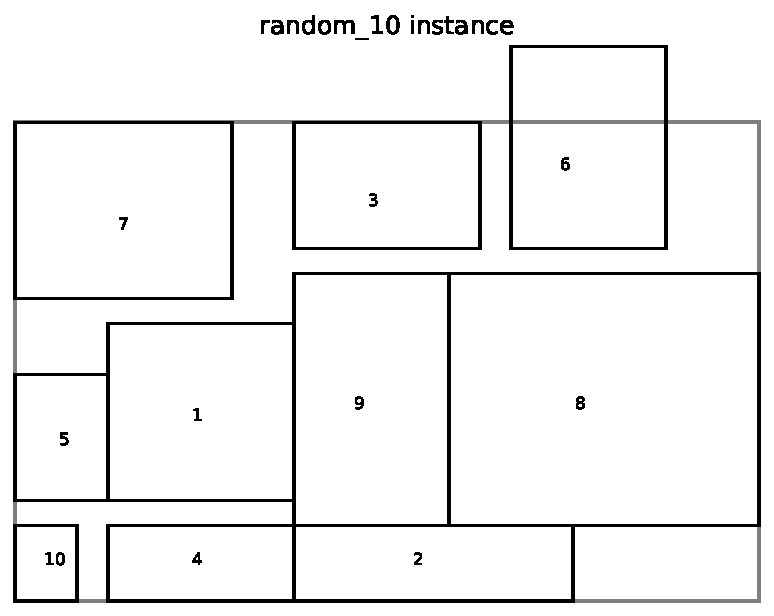
\includegraphics[width=0.8\textwidth, center]{visualizations/visualization_random_10}
    \caption
    {TODO overlappings=1}
    \label{fig:results:visualization-random-10}
\end{figure}

\begin{figure}[h!]
    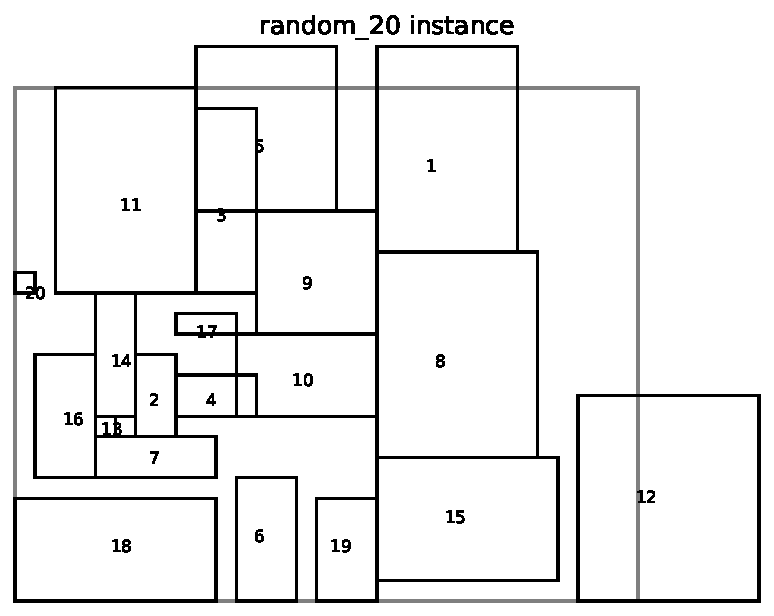
\includegraphics[width=0.8\textwidth, center]{visualizations/visualization_random_20}
    \caption
    {TODO overlappings=2}
    \label{fig:results:visualization-random-20}
\end{figure}

\begin{figure}[h!]
    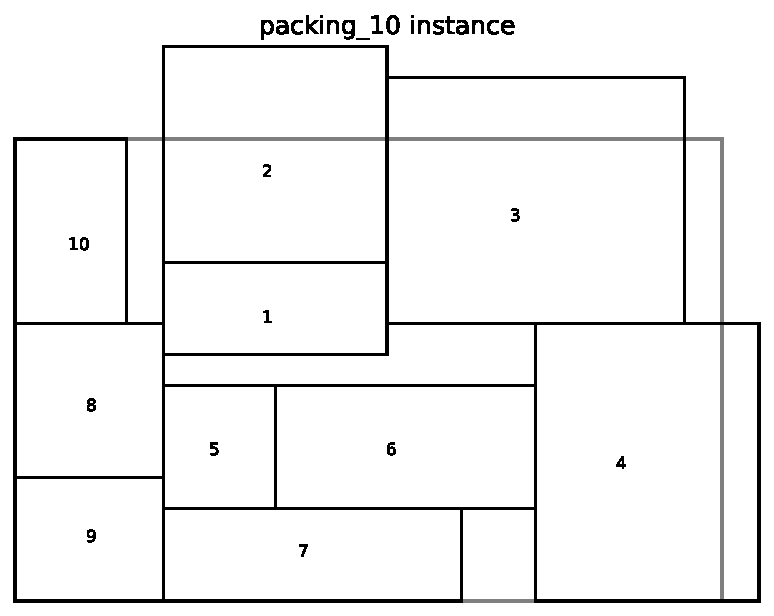
\includegraphics[width=0.8\textwidth, center]{visualizations/visualization_packing_10}
    \caption
    {TODO overlappings=0}
    \label{fig:results:visualization-packing-10}
\end{figure}

\begin{figure}[h!]
    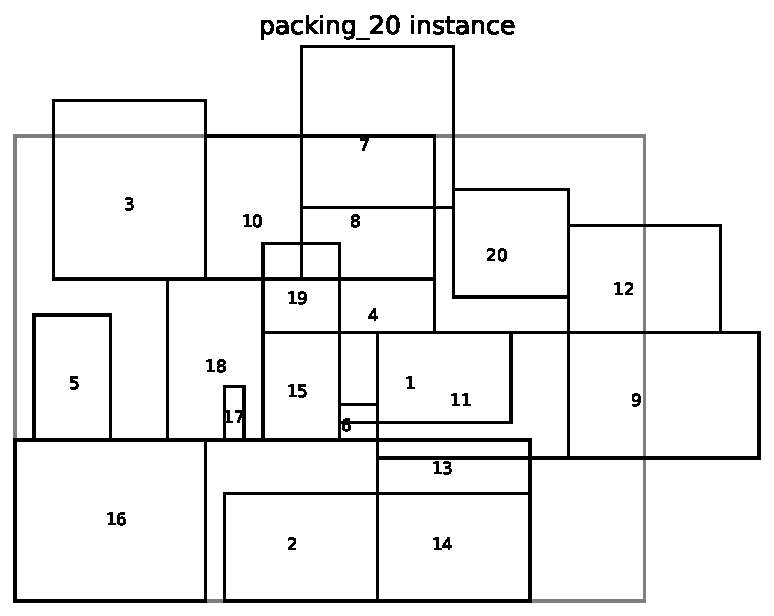
\includegraphics[width=0.8\textwidth, center]{visualizations/visualization_packing_20}
    \caption
    {TODO overlappings=8}
    \label{fig:results:visualization-packing-20}
\end{figure}

\begin{figure}[h!]
    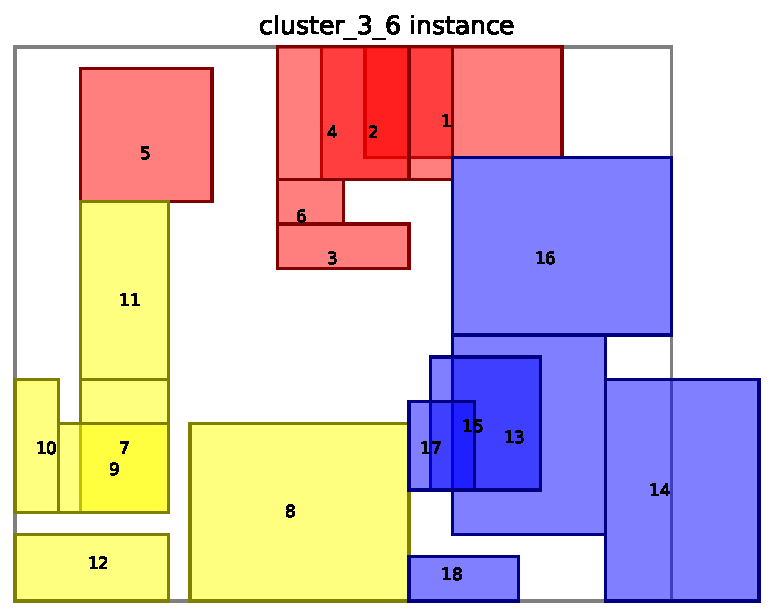
\includegraphics[width=0.8\textwidth, center]{visualizations/visualization_cluster_3_6}
    \caption
    {TODO overlappings=4}
    \label{fig:results:visualization-cluster-3-6}
\end{figure}

\begin{figure}[h!]
    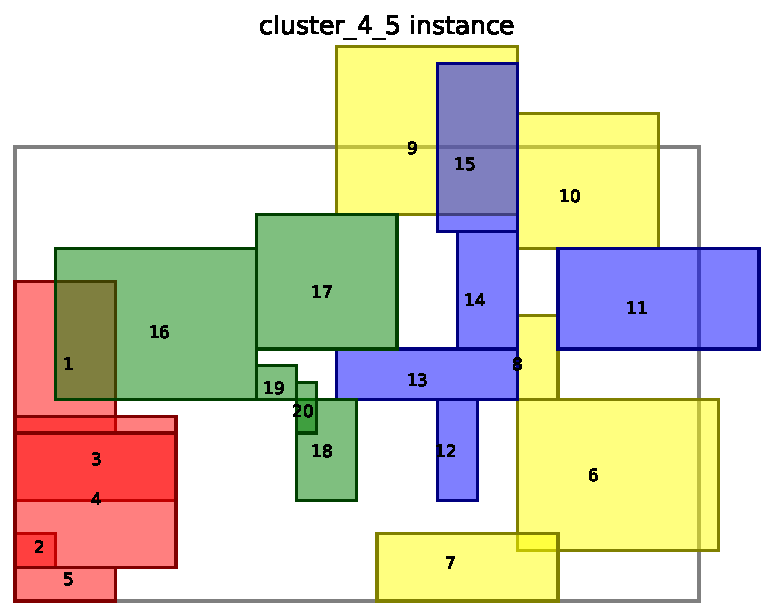
\includegraphics[width=0.8\textwidth, center]{visualizations/visualization_cluster_4_5}
    \caption
    {TODO overlappings=8}
    \label{fig:results:visualization-cluster-4-5}
\end{figure}

\begin{figure}[h!]
%    \includegraphics[width=0.8\textwidth, center]{visualizations/visualization_biased_sparse_cluster}
    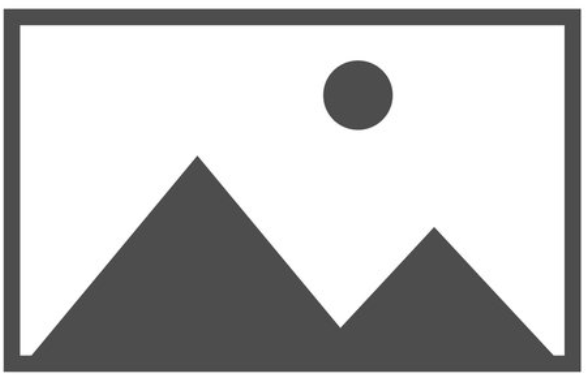
\includegraphics[width=0.8\textwidth, center]{placeholder}
    \caption
    {TODO biased sparse cluster}
    \label{fig:results:visualization-biased-sparse-cluster}
\end{figure}


\begin{figure}[h!]
    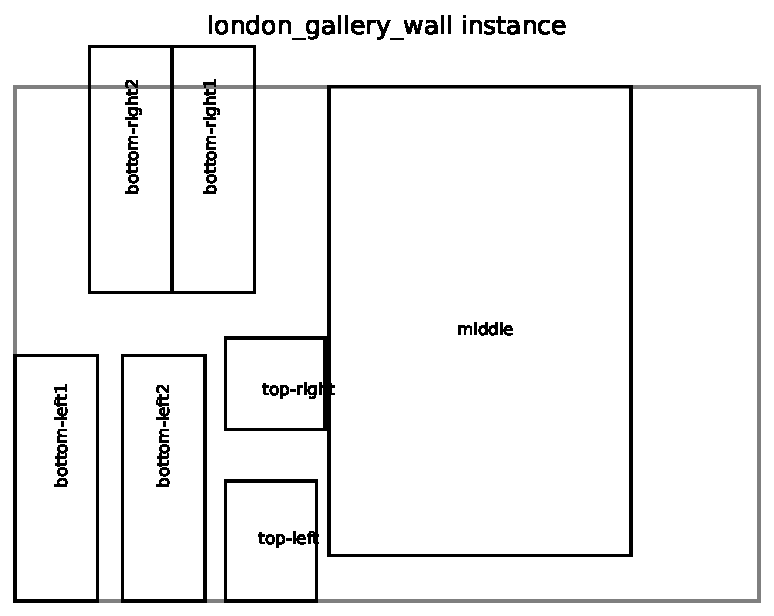
\includegraphics[width=0.8\textwidth, center]{visualizations/visualization_london_gallery_wall}
    \caption
    {TODO overlappings=0}
    \label{fig:results:visualization-london-gallery-wall}
\end{figure}


